\documentclass[12pt]{article}

% packages
\usepackage[margin=1in]{geometry}
\usepackage{graphicx}
%\usepackage{subcaption}  % needed for sub figures
\usepackage{enumerate}
\usepackage{paralist}
\usepackage{xcolor} 
\usepackage[hypcap]{caption}
%\usepackage[pdftex, colorlinks=true, linkcolor=blue]{hyperref}		% comment in final draft
\usepackage[colorlinks=false,urlbordercolor=white]{hyperref}

\usepackage[sort&compress,numbers]{natbib}
\usepackage{wrapfig}
\usepackage{subfig}


% Fonts
\usepackage[T1]{fontenc}
%\usepackage{lmodern}
\usepackage{mathptmx}
%\usepackage{fourier}
%\usepackage{tgtermes}
%\usepackage{cmbright}
%\linespread{1.1}

%%%%%%%%%%%%%%%%%%%%%%%%%%%%%%%%%%%%%%%%%%%%%%%%%%%%%%%%%%%%%%%%%%%%%%%%
% Formatting for DARPA report
%\usepackage{titlesec}
%\titleformat{\section}[runin]{\normalfont\normalsize\bfseries}{\thesection.}{1em}{}

%% indenting
%\usepackage{indentfirst}

\usepackage{titlesec}
\titleformat*{\section}{\normalsize\bfseries}
%\titleformat*{\subsection}{\normalsize\bfseries}
%\titleformat*{\subsubsection}{\normalsize\bfseries}

\titleformat{\subsection}
{\normalfont\normalsize\bfseries}{\thesubsection}{1em}{}
\titlespacing*{\subsection}{\parindent}{3.25ex plus 1ex minus .2ex}{1.5ex plus .2ex}

\titleformat{\subsubsection}[runin]
{\normalfont\normalsize\bfseries}{\thesubsubsection}{1em}{}
\titlespacing*{\subsubsection}{\parindent}{3.25ex plus 1ex minus .2ex}{1.5ex plus .2ex}


%\newcounter{DarpaSecCounter}
%\setcounter{DarpaSecCounter}{0}
%%\newcommand{\rsection}[1]{\stepcounter{DarpaSecCounter}\vspace{15pt}\noindent\textbf{{\theDarpaSecCounter.} #1}\vspace{3pt}}
%\renewcommand{\section}[1]{\stepcounter{DarpaSecCounter}\vspace{15pt}\noindent\textbf{{\theDarpaSecCounter.} #1}\vspace{3pt}}
%
%
%\newcounter{DarpaSubSecCounter}[DarpaSecCounter]
%%\setcounter{DarpaSubSecCounter}{1}
%%\newcommand{\rsubsection}[1]{\stepcounter{DarpaSubSecCounter}\indent\textbf{\theDarpaSubSecCounter. #1}}
%\renewcommand{\subsection}[1]{\vspace{4pt}\stepcounter{DarpaSubSecCounter}\indent\textbf{\theDarpaSecCounter.\theDarpaSubSecCounter. #1.}}
%
%\newcounter{DarpaSubSubSecCounter}[DarpaSubSecCounter]
%\renewcommand{\subsubsection}[1]{\vspace{2pt}\stepcounter{DarpaSubSubSecCounter}\indent\textbf{\theDarpaSecCounter.\theDarpaSubSecCounter.\theDarpaSubSubSecCounter.} \emph{#1}}

%%%%%%%%%%%%%%%%%%%%%%%%%%%%%%%%%%%%%%%%%%%%%%%%%%%%%%%%%%%%%%%%%%%%%%%%


\usepackage{amsmath}
\usepackage{amsthm}
\usepackage{amsfonts}
\usepackage{amssymb}
%\usepackage{mathrsfs}  % nice script fonts
\usepackage{mathtools}
\usepackage{bm} % bold math
%\usepackage{bbm} % blackboard math \mathbbm
%\usepackage{stix}



% Quick math font modification
\newcommand{\mc}{\mathcal}
\newcommand{\msf}{\mathsf}
%\newcommand{\mbf}{\bm} 			% requires amsmath, amssymb packages
\newcommand{\mbf}{\mathbf} 			% requires amsmath, amssymb packages
\newcommand{\mbb}{\mathbb}  	% requires bbm
\newcommand{\mf}{\mathfrak}
\newcommand{\mscr}{\mathscr}

% Spaces
\newcommand{\N}{ \ensuremath{\mathbb{N}}}  % natural numbers
\newcommand{\Z}{ \ensuremath{\mathbb{Z}}}  % integers
\newcommand{\Q}{ \ensuremath{\mathbb{Q}}}
\newcommand{\R}{ \ensuremath{\mathbb{R}}}  % real numbers
\newcommand{\C}{ \ensuremath{\mathbb{C}}}  % complex numbers
\newcommand{\K}{ \ensuremath{\mathbb{K}}}  % scalar field \R or \C
\newcommand{\T}{\ensuremath{\mathbb{T}}}
\newcommand{\D}{ \ensuremath{\mathbb{D}}}

% Short-hand greek
\newcommand{\eps}{\epsilon}
\newcommand{\del}{\delta}
\newcommand{\lam}{\lambda}
\newcommand{\al}{\alpha}

% set theory
\providecommand\given{} % make sure it exists
\newcommand\SetSymbol[1][]{
   \nonscript\,#1\vert \allowbreak \nonscript\,\mathopen{}}

\DeclarePairedDelimiterX\set[1]{\lbrace}{\rbrace}{ \renewcommand\given{\SetSymbol[\delimsize]} #1 }  % set* autoscales
\newcommand{\Union}{\bigcup} 		% big union
\newcommand{\union}{\cup} 			% little union
\DeclareMathOperator{\inter}{int}

% Vector spaces/ Operators
\DeclarePairedDelimiterX\norm[1]{\lVert}{\rVert}{#1}  			% norm (\norm*{} autoscales or \norm[\big]{})
\DeclarePairedDelimiterX\inner[2]{\langle}{\rangle}{#1 \,,\, #2}  	% inner product
\newcommand{\transp}{\mathsf{T}}  								% transpose
\DeclareMathOperator{\linspan}{span} 							% linear span
\DeclareMathOperator{\rank}{rank}								% Rank of a matrix.
\DeclareMathOperator{\diag}{diag}								% Diagonal matrix.
\newcommand{\Null}{N}  											% Nullspace
\newcommand{\Ran}{Ran}											% Range
\DeclareMathOperator{\image}{Im}								% Image
%\newcommand{\closure}[1]{\overline{#1}}							% Closure

% math functions
\DeclarePairedDelimiterX\abs[1]{\lvert}{\rvert}{#1} % absolute value: \abs{} = no-resize, \abs*{} = left/right auto-resize, \abs[size-cmd]{} = size manually adjusted with size-cmd = \big,\Big,\bigg,\Bigg
\DeclareMathOperator{\sign}{sgn}
\newcommand{\one}{ \ensuremath{\bm{1}}}
\DeclareMathOperator{\supp}{supp}								% Support
%\newcommand{\ind}[1]{\mathbb{I}_{#1}}							% indicator function
\newcommand{\ind}[1]{\mathbbm{1}_{#1}}							% indicator function
\newcommand{\ud}{\,d}  % differential with space before symbol

% Theorem environments
\theoremstyle{plain}
  \newtheorem{theorem}{Theorem}[section]
  \newtheorem{lemma}[theorem]{Lemma}
  \newtheorem{proposition}[theorem]{Proposition}
  \newtheorem{conjecture}[theorem]{Conjecture}
  \newtheorem{claim}[theorem]{Claim}
  \newtheorem{myquestion}[theorem]{Question}
  \newtheorem*{corollary}{Corollary}
\theoremstyle{remark}
  \newtheorem*{remark}{Remark}
  \newtheorem*{remarks}{Remarks}
  \newtheorem*{justification}{Justification}
\theoremstyle{definition}
  \newtheorem{example}[theorem]{Example}
  \newtheorem{definition}[theorem]{Definition}
  \newtheorem*{notation}{Notation}


% annotate
\newcommand{\blue}[1]{{\color{blue} #1}}
\newcommand{\red}[1]{{\color{red} #1}}
\newcommand{\needcite}{{\tiny\blue{need citation}}}
\newcommand{\todo}[1]{{\tiny\red{#1}}}

% paper-specific definitions
\newcommand{\mat}[1]{\mbf{#1}}  % font style for matrices
\newcommand{\op}[1]{\mathcal{#1}}  % font style for operators
\newcommand{\vsp}[1]{\mathsf{#1}}  % font style for vector spaces
\newcommand{\size}[1]{\mathrm{size}(#1)}
\newcommand{\up}{\uparrow}
\newcommand{\dn}{\downarrow}

\newcommand{\Ko}{C}  % Koopman operator
\newcommand{\Kdm}{A}  % Koopman diffusion operator (asymmetric kernel)
\newcommand{\Dm}{D}  % Diffusion operator (symmetric kernel)
\newcommand{\psdm}{p_{\sigma,\delta}^{(m)}}

\usepackage{lipsum}

\renewcommand{\r}{\bm{p}}
\newcommand{\units}[1]{\mathsf{#1}}


\newcommand{\bmat}[1]{\begin{bmatrix} #1 \end{bmatrix}} % short hand bracket matrix
\newcommand{\pmat}[1]{\begin{pmatrix} #1 \end{pmatrix}} % short hand bracket matrix

\newcommand{\rmm}[1]{{\color{red}#1}}

\renewcommand{\vec}[1]{\mathbf{#1}}

\newcommand{\x}{\mathbf{x}}

\newcommand{\email}[1]{\href{mailto:#1}{\color{blue}\underline{#1}}}

% MHG packages
\usepackage[version=3]{mhchem}
\usepackage{braket}
\usepackage{relsize}
%\usepackage{enumitem}
%\usepackage[vlined]{algorithm2e}
%\usepackage{algpseudocode}
%\usepackage[font=small,labelfont=bf]{caption}
%\usepackage{graphicx}
%\usepackage{footnote}
%\usepackage{multirow}
%\usepackage{tabularx}
\usepackage{booktabs}
\usepackage{makecell}
\usepackage{threeparttable}
\usepackage{chemfig}
\usepackage{siunitx}

%========================================================================
\begin{document}

%========================================================================

% == Accomplishments during reporting period

\section{Executive summary}

\begin{figure}
	\centering
	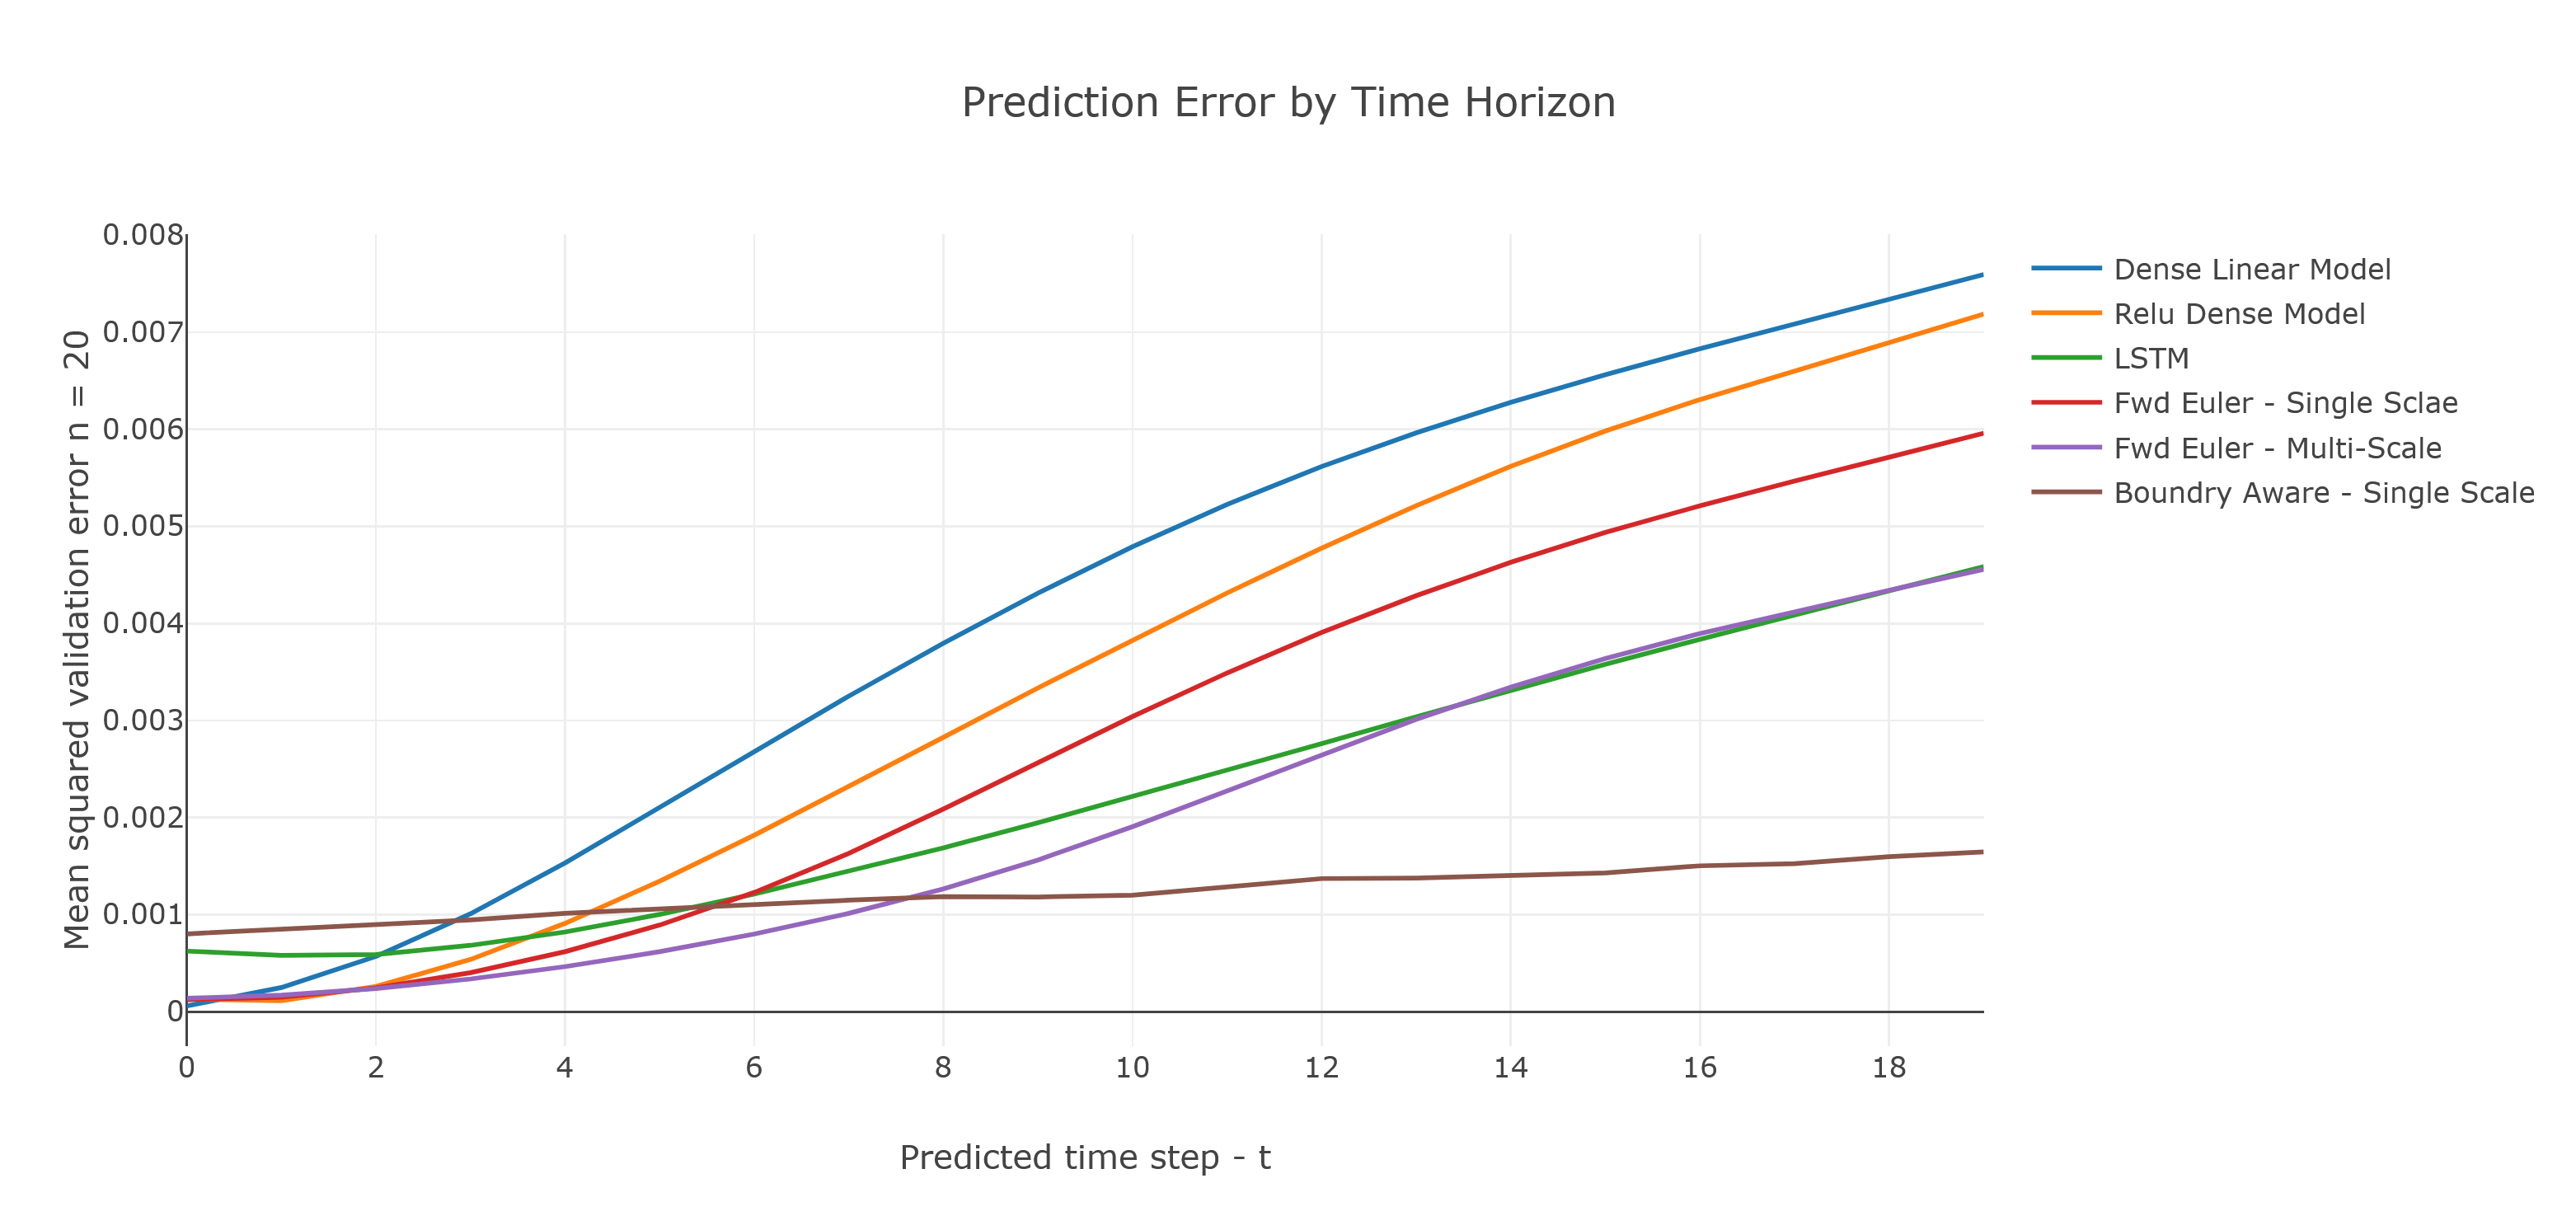
\includegraphics[width=0.95\linewidth]{performance_boundry_aware}
	%	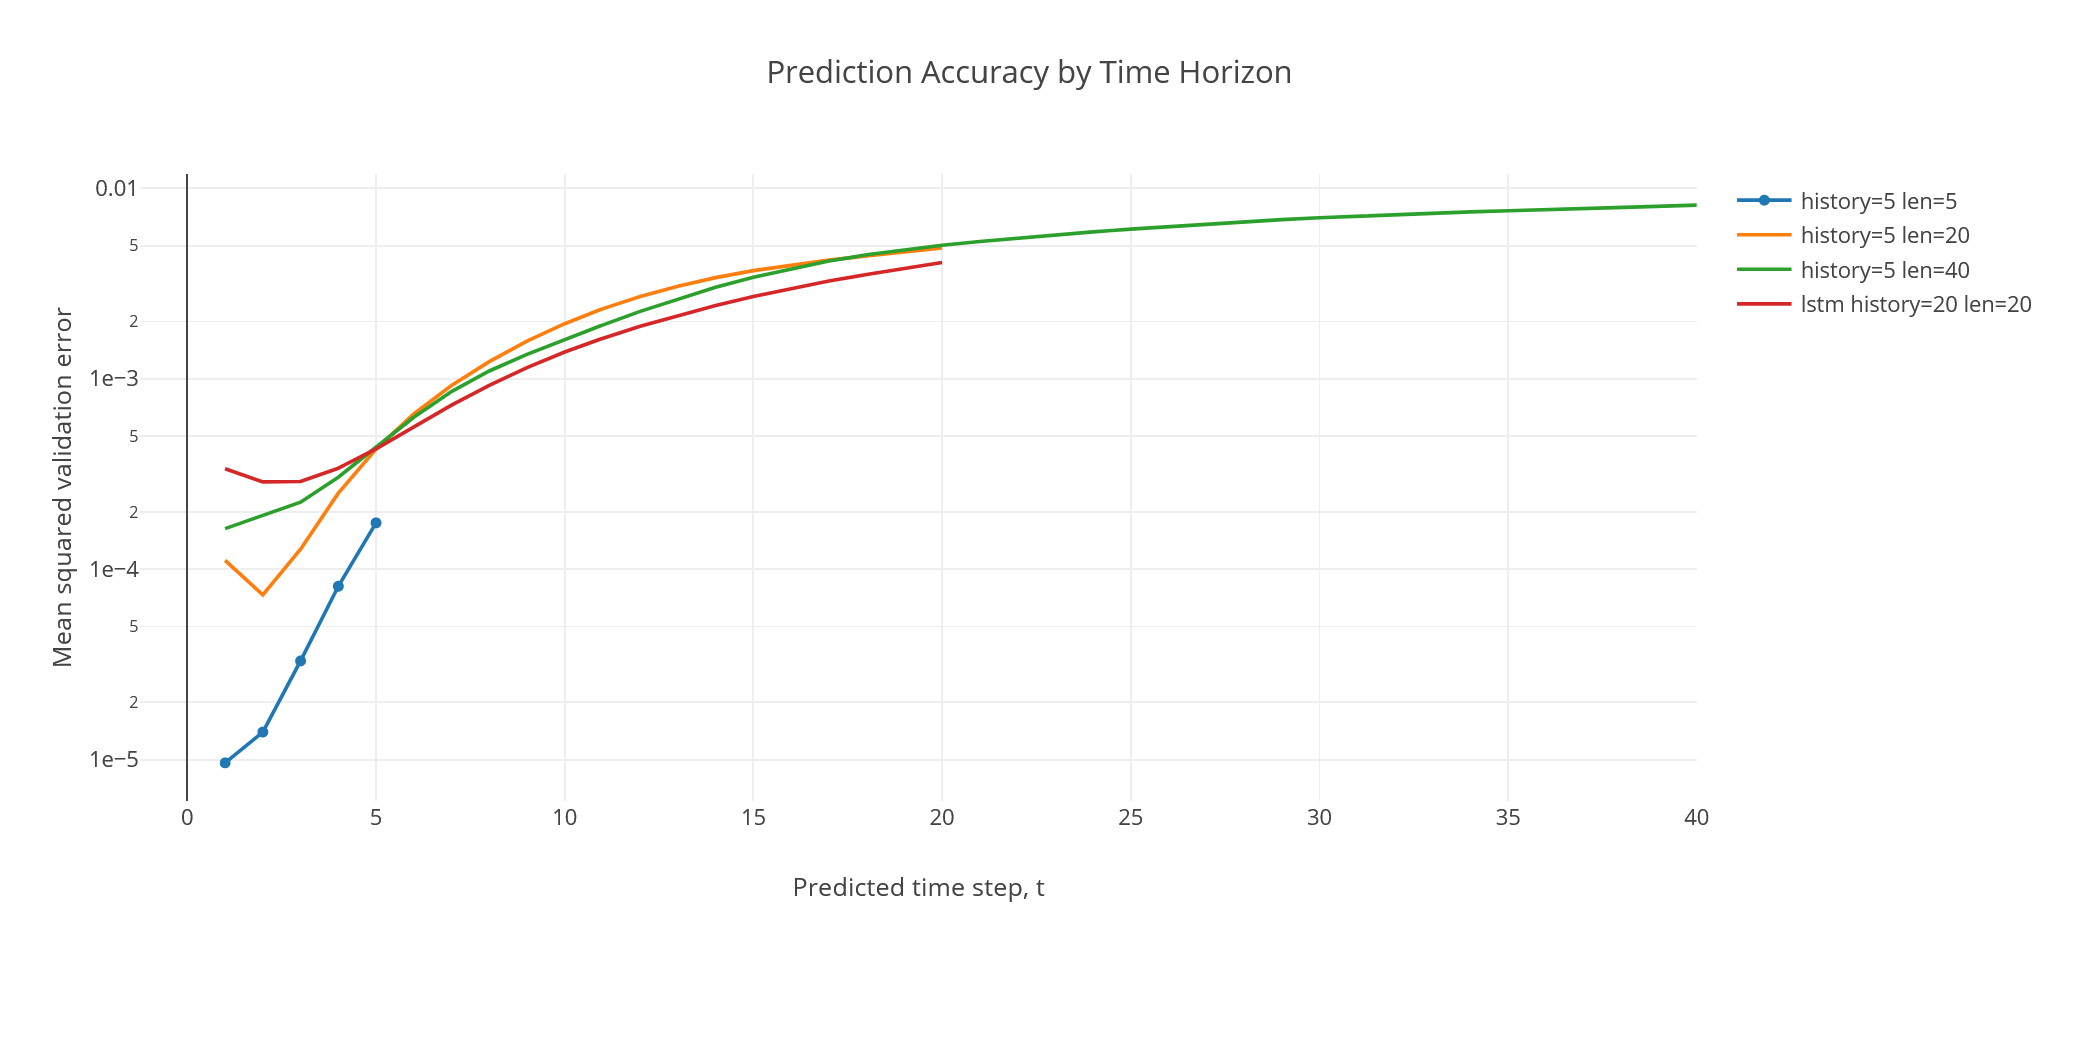
\includegraphics[width=0.9\linewidth]{pde_perf_linear}
	\caption{\small Mean squared error by predicted time-step. Note the strong consistency in accuracy over time offered by the boundary-aware architecture.}
	\label{fig:perf_over_time}
\end{figure}	



\begin{figure}
	\centering
	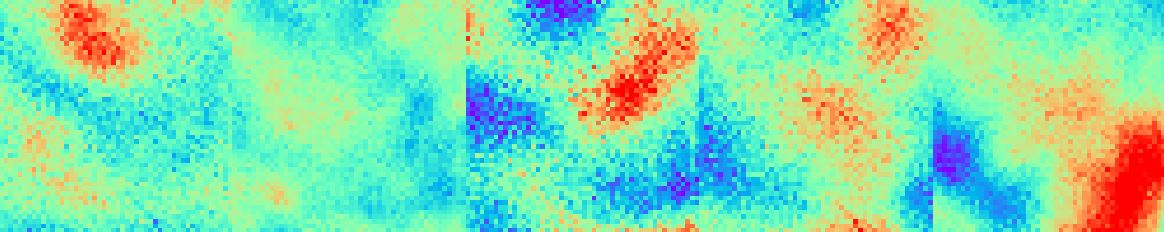
\includegraphics[width=0.95\linewidth]{low_frequency_noise}
	%	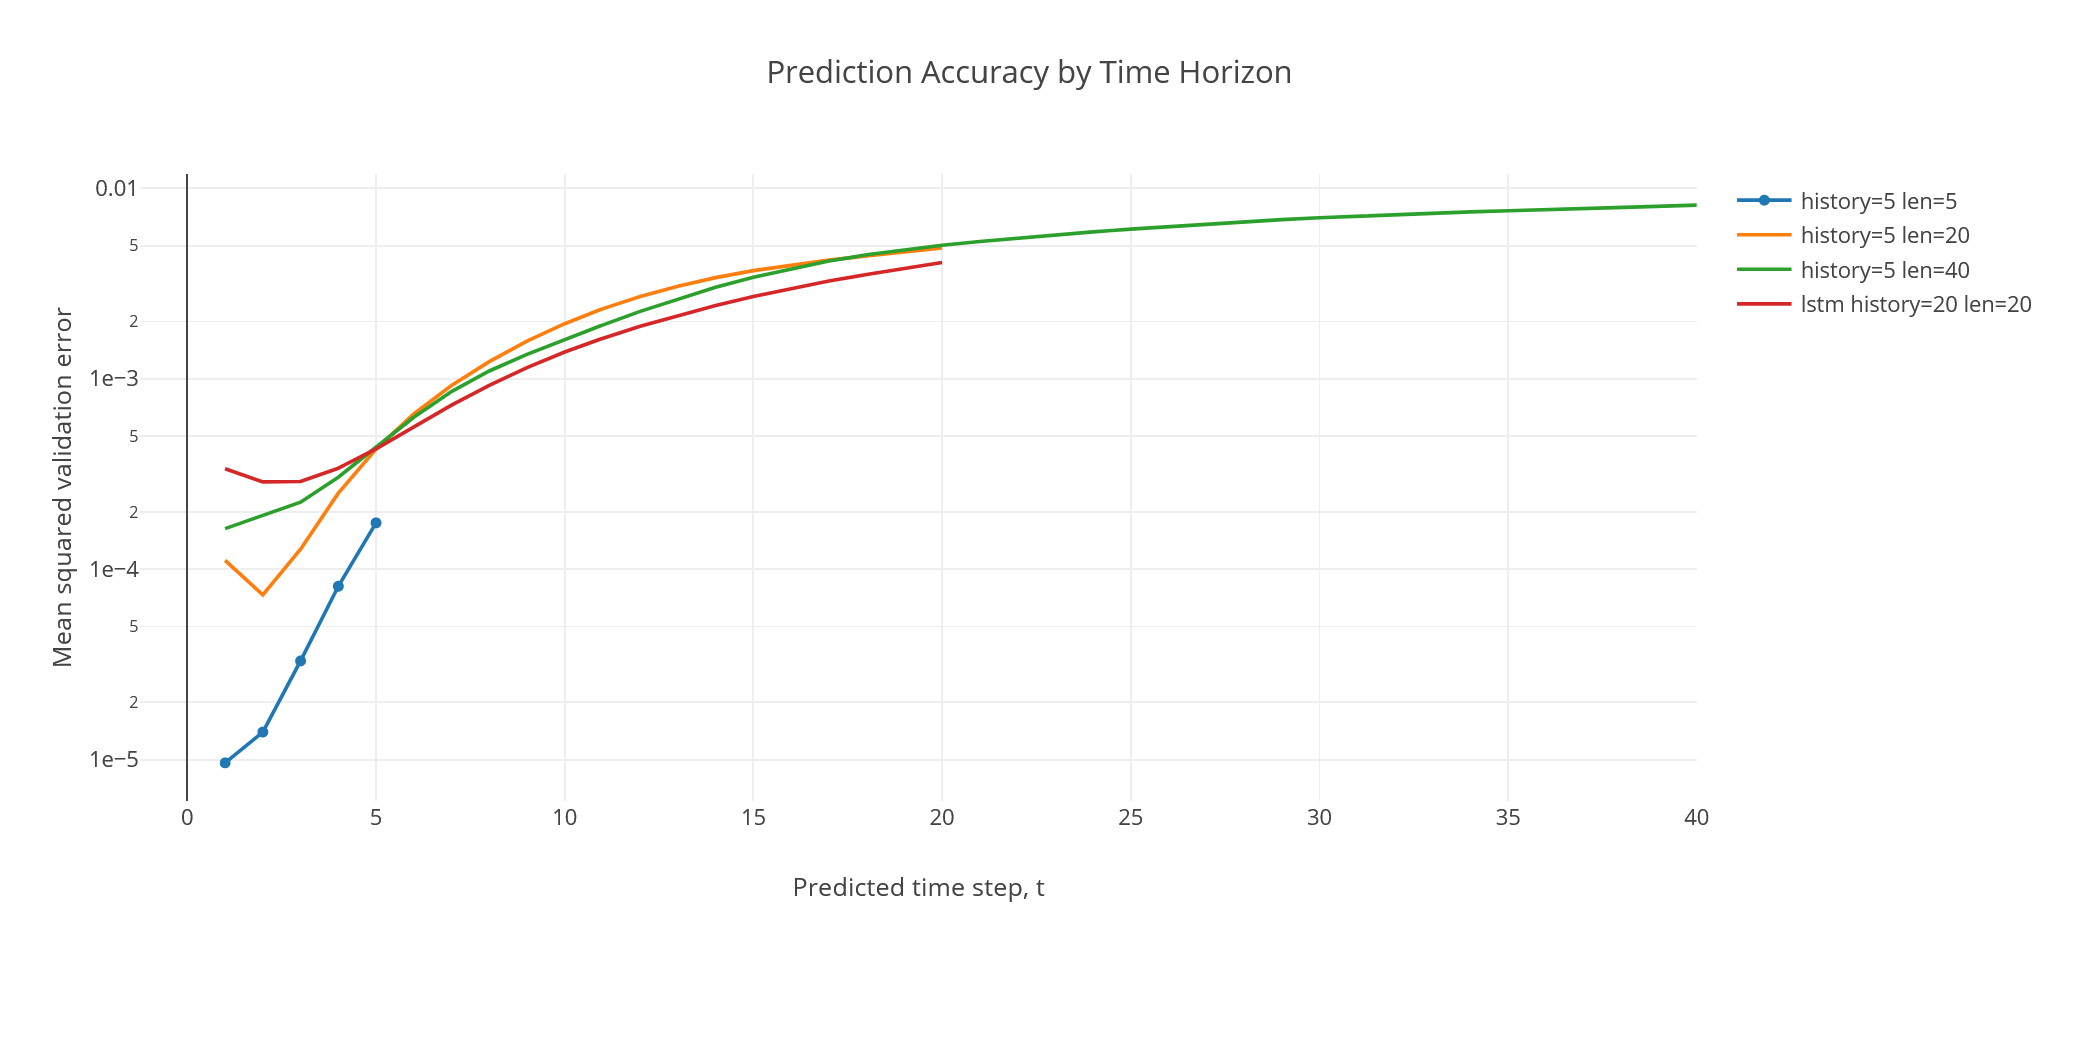
\includegraphics[width=0.9\linewidth]{pde_perf_linear}
	\caption{\small Visualization of prediction error $\hat{y} - y$ at $t=20$ for baseline linear model. While early time-step accuracy is high, prediction degrades quickly as shown in figure \ref{fig:perf_over_time}. }
	\label{fig:low_frequency_noise}
\end{figure}

\begin{figure}
	\centering
	
\includegraphics[width=0.95\linewidth]{high_frequency_noise}
	%	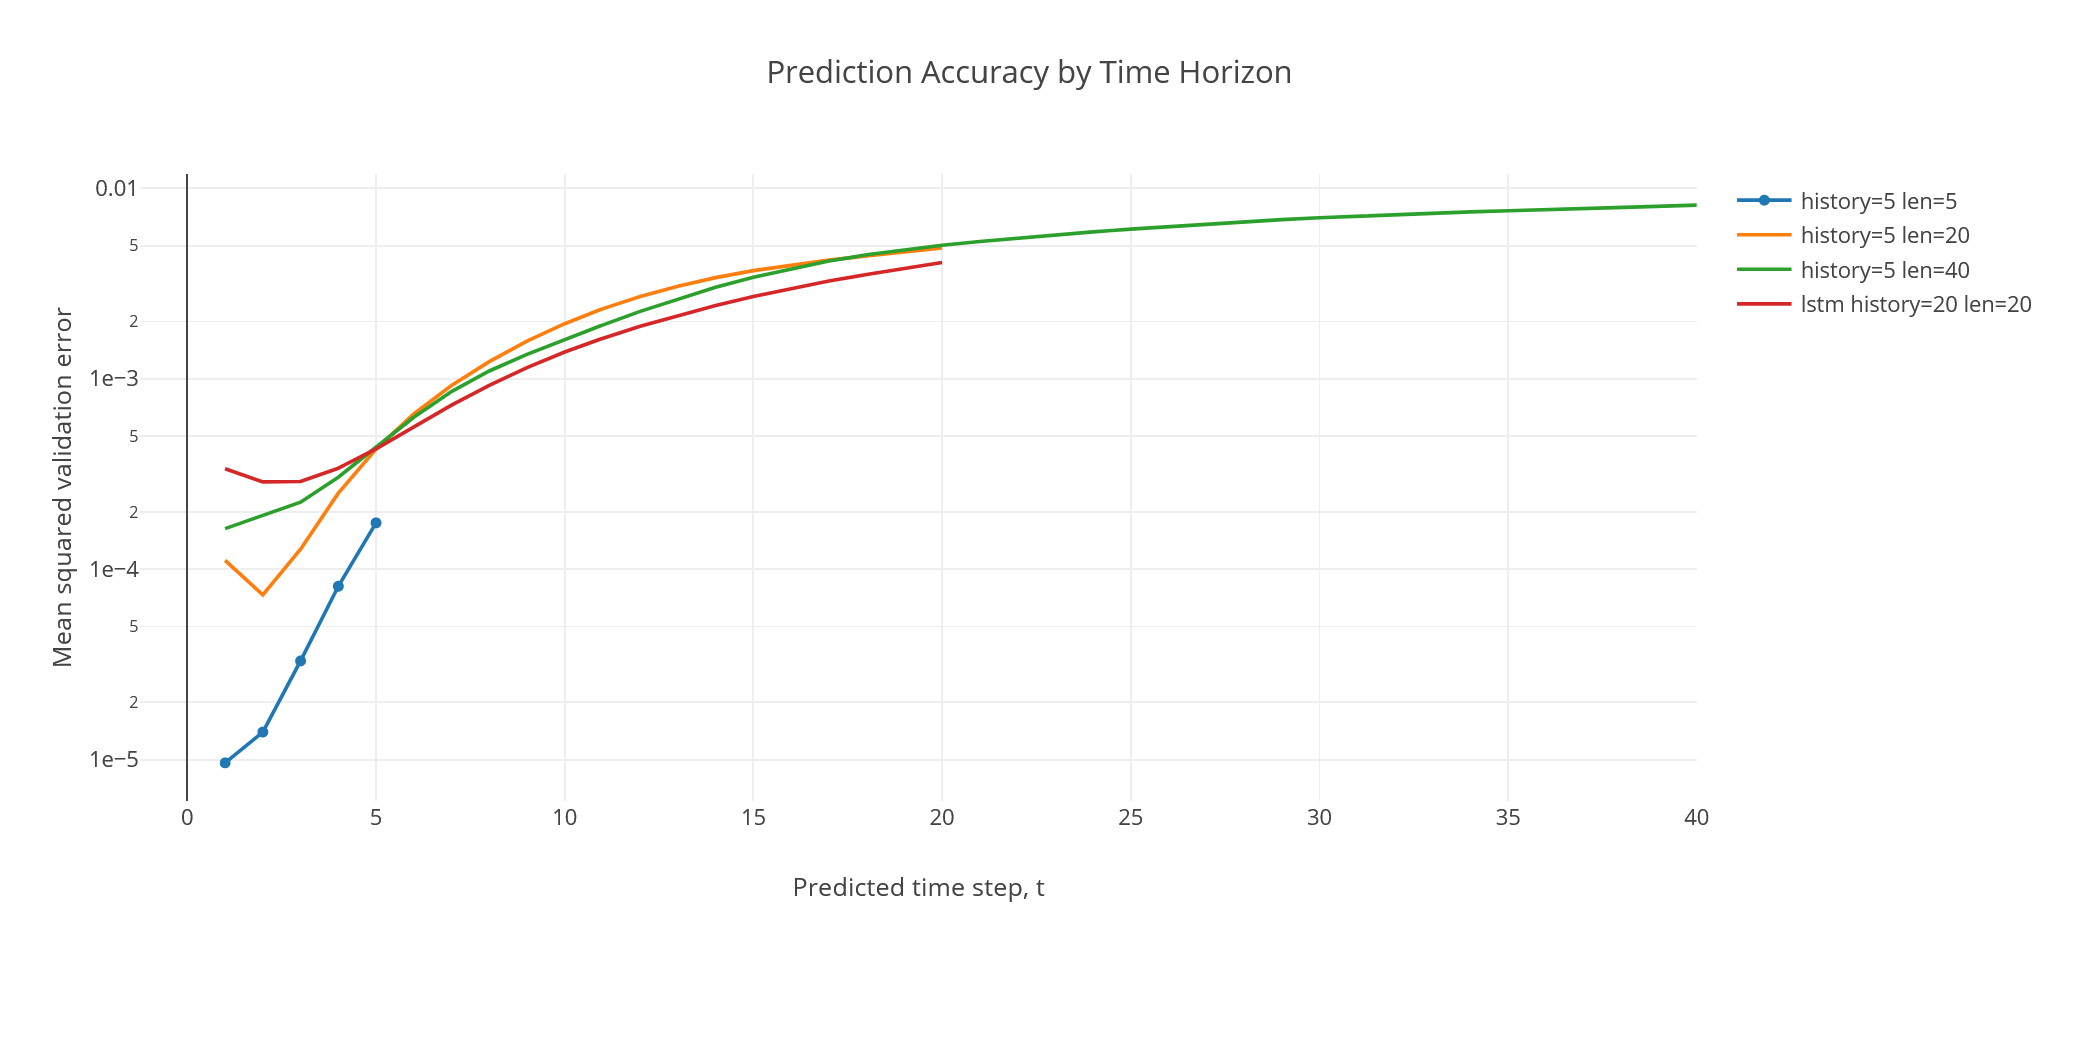
\includegraphics[width=0.9\linewidth]{pde_perf_linear}
	\caption{\small Visualization of prediction error $\hat{y} - y$ at $t=20$ for the boundary-aware prediction model. Note that compared to previous approaches, boundary-aware architectures resolve low-frequency, long-term dynamics more accurately across the entire predicted trajectory as shown in figure \ref{fig:perf_over_time}. }
	\label{fig:high_frequency_noise}
\end{figure}	

\begin{figure}
	\centering
	
\includegraphics[width=0.2\linewidth]{conv_error}
	\caption{Mean prediction error over a batch of patches for the forward-Euler single scale architecture. Note the artifacts along the edge of the region resulting from estimating boundary state.}
	\label{fig:conv_mean_error}
\end{figure}



\subsection{Previous work}

Previous work significantly improved performance of discovered architectures, using deep, multi-scale convolutions to learn complex dynamics efficiently in terms of network parameters. Additionally we developed a curriculum learning style approach, varying the prediction horizon leveraging temporal consistency of turbulent dynamics to further increases in network performance and robustness during training. Finally, we established a benchmark metric, based on relative accuracy as compared to a linear baseline, dubbed $RBA$, where perfect prediction represents a score of 1, and 0 indicates baseline mean-squared error.



\subsection{Important Results}
In this period, we addressed spatially inconsistent boundary conditions by developing a new boundary-aware network architecture. This boundary-aware architecture further reduces mean squared error by 56\% as compared to the previous best performing forward-Euler, multi-scale model, while maintaining an accurate prediction ($MSE_t < 0.002$) for the entire trajectory. While previous architectures have struggled with accumulation of error near the edges of predicted patches as shown in figure \ref{fig:conv_mean_error} \textcolor{blue}{ and compounding systematic error in predicting long-term dynamics as seen in figure \ref{fig:low_frequency_noise}}, the new architecture shows uniform error over the entire prediction region. This uniform error is illustrated by the comparatively gentle slope of the brown boundary aware architecture line in figure \ref{fig:perf_over_time} and the uniform, low-magnitude, high-frequency error in figure \ref{fig:high_frequency_noise}.
 

\begin{table}[]
	\centering
	\begin{tabular}{llll}
		& MSE       & RBA    &  \\
		Linear Baseline              & 0.004356  & $\sim$ &  \\
		Fully Connected              & 0.003694  & 0.2374 &  \\
		LSTM                         & 0.002326  & 0.3583 &  \\
		Foward Euler - Single Scale  & 0.002971  & 0.3857 &  \\
		Forward Euler - Multi Scale  & 0.002116  & \textbf{0.5483} &  \\
		Boundary Aware               & \textbf{0.000922}  & 0.4351 & 
	\end{tabular}
	\caption{Comparison of network accuracy over 20 time-steps. Despite lower mean squared error, the boundary aware architecture has a lower RBA than multi-scale forward-Euler given its disadvantage over the baseline in early time-steps.}
	\label{table:performance}
\end{table}

\subsection{Hypothesis 1 - Boundary-Aware Architectures}

Previously, the forward Euler inspired \textcolor{blue}{architecture, illustrated in figure \ref{fig:arch_multi},} leveraged convolutions at multiple scales to increase the fidelity of the dynamics model while maintaining the symmetry-constrained properties of a convolutional architecture. However, these architectures are sensitive to changing boundary conditions because of the nature of convolutional layers incorporating local features which are not present on boundaries. This effect is compounded when \textcolor{blue}{convolution is} repeatedly applied as is the case when rolling out predictions. When applying the dynamics across the entire flow, rather than discrete regions of turbulence, boundary conditions would be fixed at the physical borders, and therefore predictable and possible to estimate. However, given the patch formulation we see previously models unable to approximate boundary conditions which caused systematic error along borders as seen in figure \ref{fig:conv_mean_error}.

To address this, we develop so called boundary-aware architectures that enforce boundary conditions during prediction roll-outs. This maintains the architectural assumption of spatially consistent dynamics, and grounds predictions by assuming true dynamics are known at patch edges. This architecture, illustrated in figure \ref{fig:boundry_aware_arch} dramatically increased prediction accuracy, especially over distant time-steps where compounding errors typically preclude accurate prediction.


\subsubsection{What was to be tested? What was the expected outcome prior to testing?}
	We tested constraining networks by padding the previous state $\hat{x}_t$ with ground truth boundary conditions $x_t$. We expected this to increase long-term prediction accuracy by eliminating compounding errors along boundaries, though by directly padding previous state with boundary conditions, this requires a different approach then previous network architectures as the dynamics are learned directly, rather than learning the dynamics of a hidden state,$u_t$.
	%We test the addition of convolutional features at different scales to learn the problem dynamics more accurately. The resulting architecture is illustrated in figure \ref{fig:arch_multi}. Previous architectures used only a single scale for convolutional features meaning the network had access to only local information. By adding multiple scales to the dynamics update we hope to enable the network to learn to use both local and global features in the region to predict more accurately.


\subsubsection{High-level summary of main results.}
Using boundary-aware architectures, we were able to reduce MSE by 54\% and decrease error-accumulation by a factor of 6. Further architecture improvements will likely lower MSE further given high relative MSE for early $t < 3$ time-steps.
	%We see strong performance gains by the addition of the additional scales. As shown in figure \ref{fig:pdeperf}, for the multi-scale architecture prediction is accurate over both the short-term and long-term predictions, beating LSTM based methods in short-term prediction.  


\subsubsection{Discuss relevance to project and DARPA concerns.}
This represents a significant improvement in long-term dynamics modeling for turbulent flow. The accumulation of compounding error can quickly cause predictions to diverge, however this approach has shown to reduce this compounding error accumulation by a factor of 6 enabling the simulation of long-term dynamics potentially 6x further into the future.
%	In numeric PDE solvers, choosing the proper simulation scale can dramatically effect the accuracy of simulations even for known PDEs. Given the increase in performance we see that with the addition of multi-scale convolutional layers, networks learn the proper scale for accurate prediction dynamically. This results in networks that are general and adapt well to new problems.




%========================================================================
\section{Achievements}

\subsection{Scientific Breakthroughs}

None

\subsection{Technology developments}

None 

\subsection{Application results}

Boundary aware architecture decreased compounding error accumulation by a factor of 6 suggesting that longer-term prediction experiments are necessary to test the limits of turbulent vorticity projection. Previously, error beyond 20 time-steps was too large for accurate ($MSE_t < 0.002$) prediction, however current boundary -aware architectures easily maintain an accurate predicted vorticity through the entire 20 step trajectory.% 

\subsection{Transitions achieved}

None

%========================================================================
\section{Lessons Learned}


\noindent Problems encountered/risks that occurred, and corresponding solutions/mitigations

None

\noindent Open Issues

None

%========================================================================
\section{Next Steps}

\noindent Boundary-aware techniques show significant promise in extending the prediction horizon for turbulent patches. Additional architectures incorporating both multi-scale forward Euler inspired methods and boundary-aware techniques remain to be explored.

\noindent Boundary constraints eliminate network prediction of boundary conditions, which are varied given the spatial segmentation of the turbulent flow. In practice these boundary conditions may not be available for constraining predictions, therefore it is of interest to apply patch dynamics iteratively over the entire flow field using local predictions as estimated boundary conditions.

\noindent Short-term $(t < 3)$ predictions show larger than baseline mean squared error, suggesting that the network is not expressive enough to capture high-frequency features. Further experiments integrating additional network features from previous architectures are needed.


%========================================================================
\section{Technical details}

To evaluate new models in a standard way, we establish a baseline performance using a fully connected linear network, and introduce a relative baseline accuracy metric, where $\sigma$ represents the mean squared error of the model for a given time-step t.
$$RBA =  \frac{1}{n}\sum_{t=1}^{n}\frac{(y_t - \hat{y_t}_{baseline})^2 -(y_t - \hat{y_t}_{model})^2}{ (y_t - \hat{y_t}_{baseline})^2}$$ 

\begin{figure}
	\begin{minipage}[c]{0.45\textwidth}
		\centering
		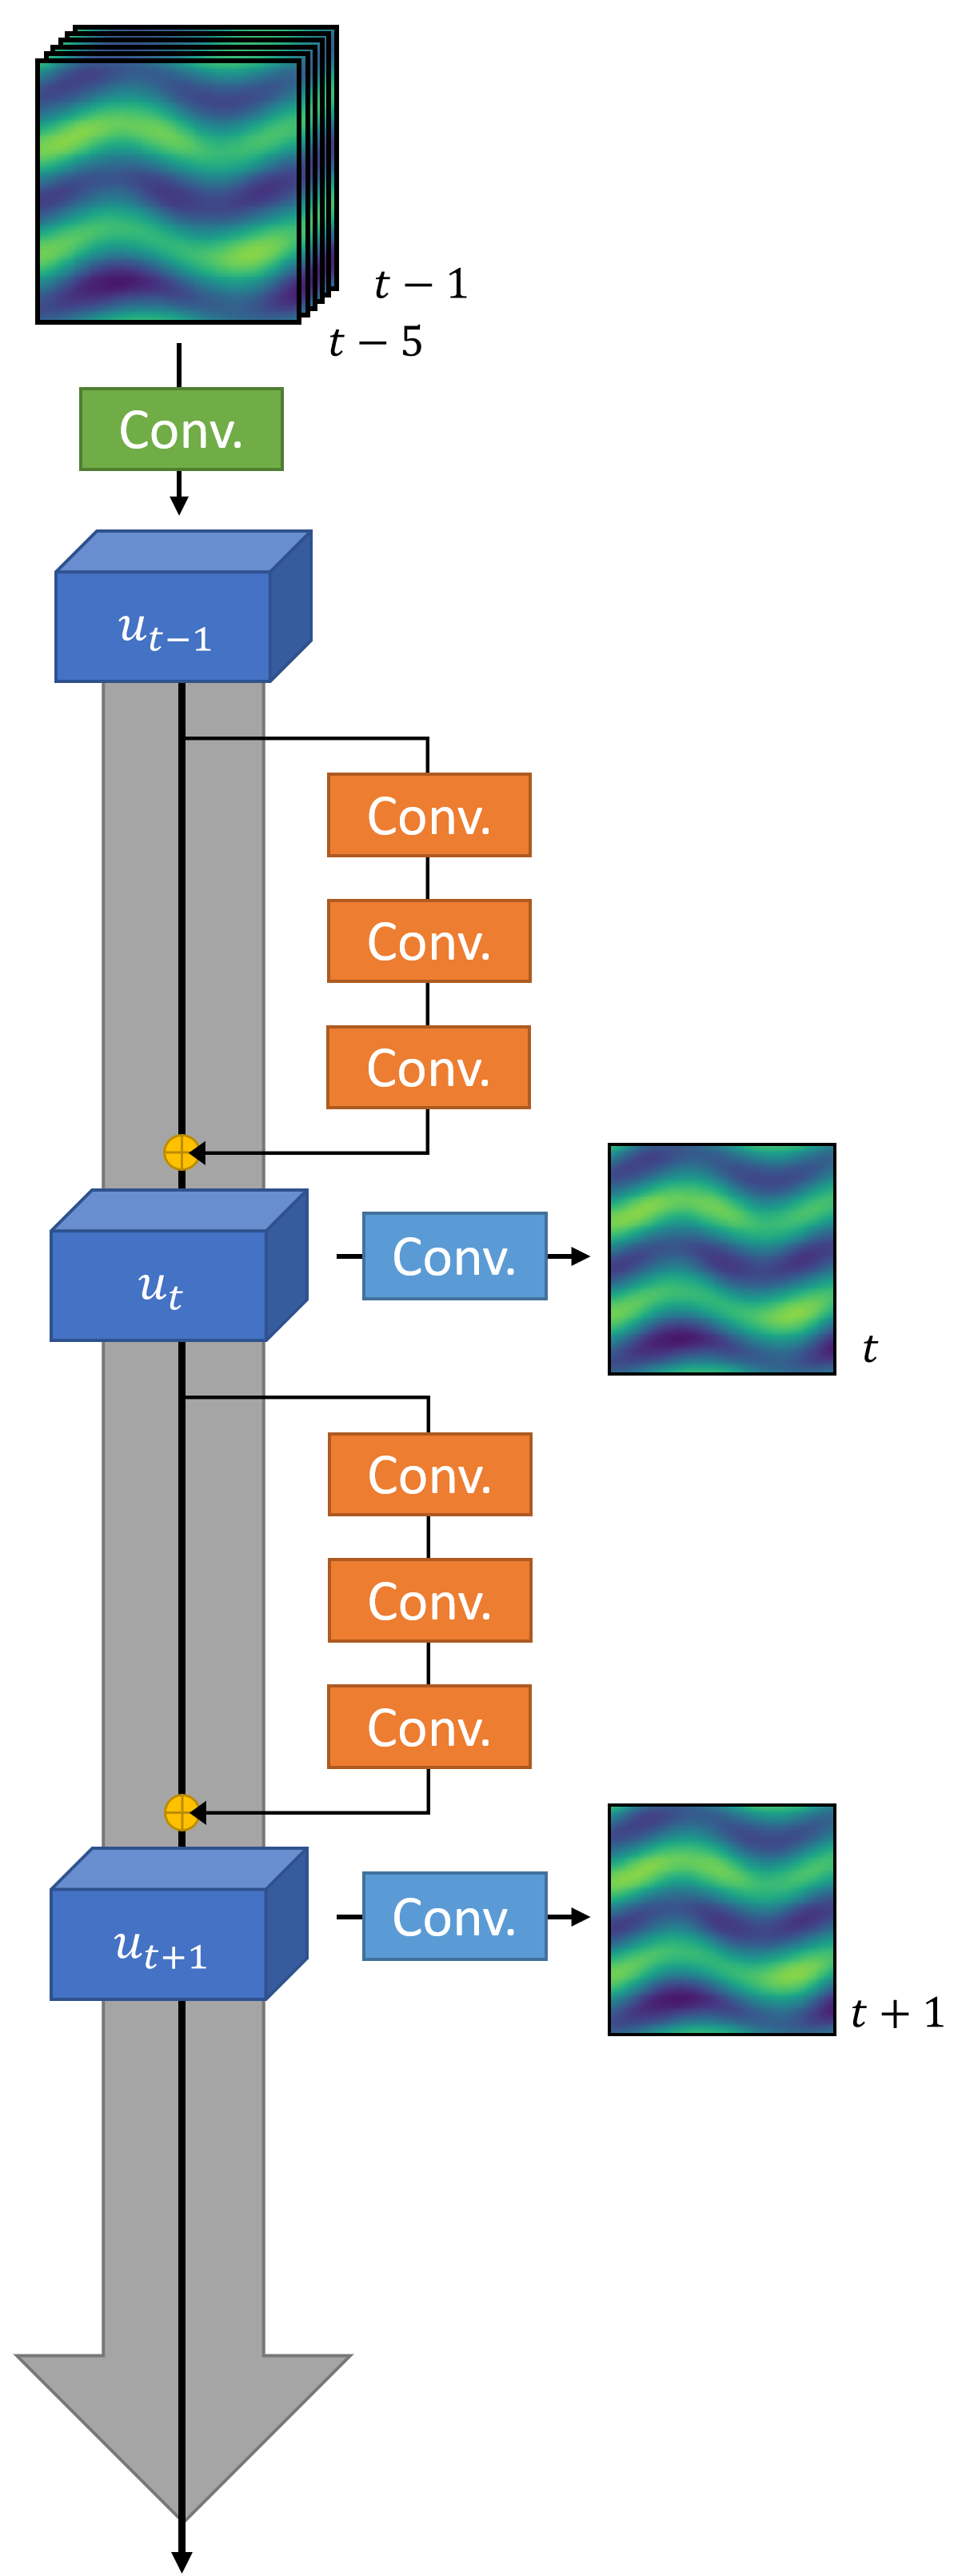
\includegraphics[width=2.5in]{pde_arch}
		\caption{Illustration of the single-scale forward Euler architecture. The encoder $\phi(x)$ (shown in green) maps the input into the feature space. Three convolutional layers (shown in orange) are used to approximate the feature space dynamics $f(u_t)$ and summed with $u_t$ (shown in yellow) to give $u_{t+1}$ as outlined in equation \ref{eqn:ode}. At each step, the feature vector $u_t$ is decoded by $\theta(u_t)$ (as shown in light blue) predicting $x_{t+1}$.}
		\label{fig:arch}

	\end{minipage}
	\hspace{0.1\textwidth}
	\begin{minipage}[c]{0.45\textwidth}
		\centering
		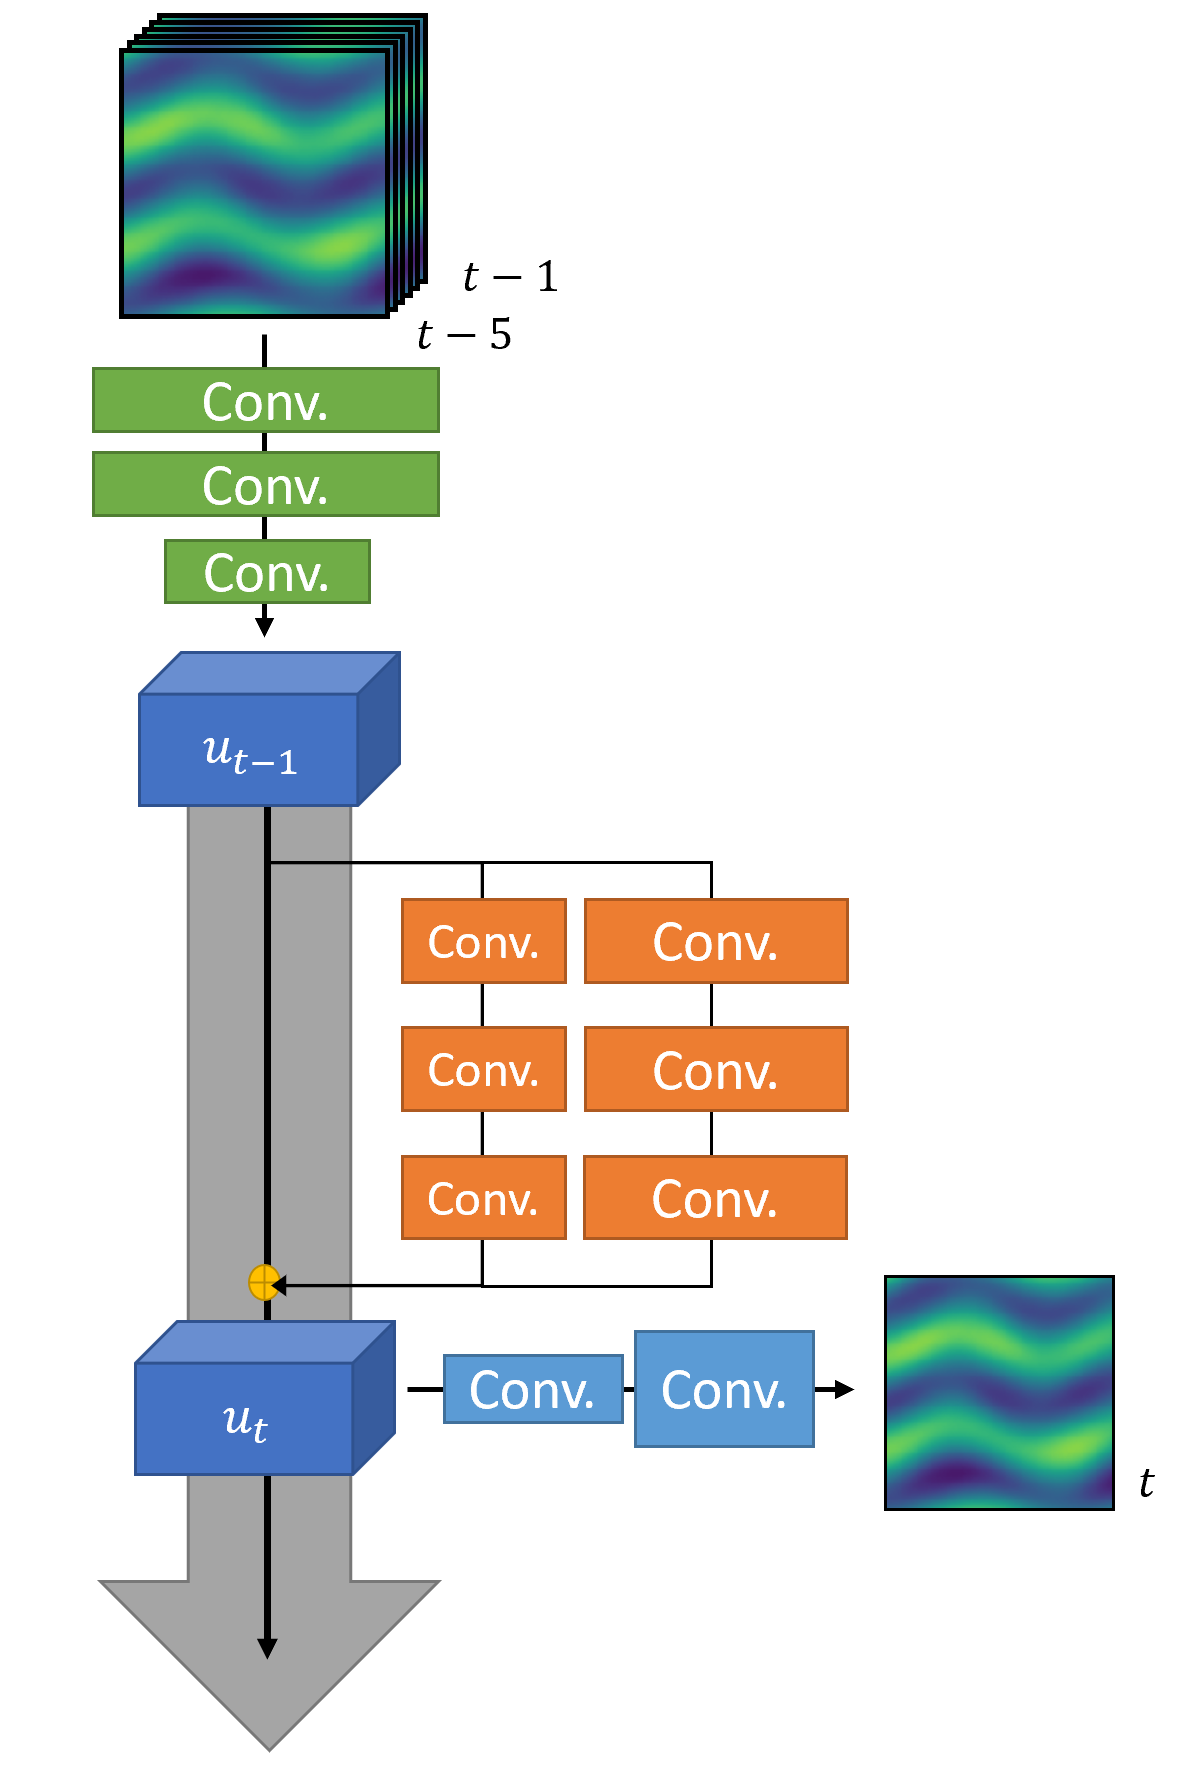
\includegraphics[width=2.75in]{pde_arch_multi}
		\caption{Illustration of the multi-scale forward Euler architecture. The
		dynamics $f(u_t)$ are enriched with filters at different scales (shown in orange). Additionally, the encoder $\phi(x)$ reduces the dimensionality of the input image by a factor of 4 in the encoding step $\phi(x)$ to increase the receptive field of the dynamics update calculation, $f(u_t)$ allowing for lower frequency features to be captured by the network. }
		\label{fig:arch_multi}
	\end{minipage}
\end{figure}



\subsection{Boundary-Aware architectures}

\begin{figure}
	
	\centering
	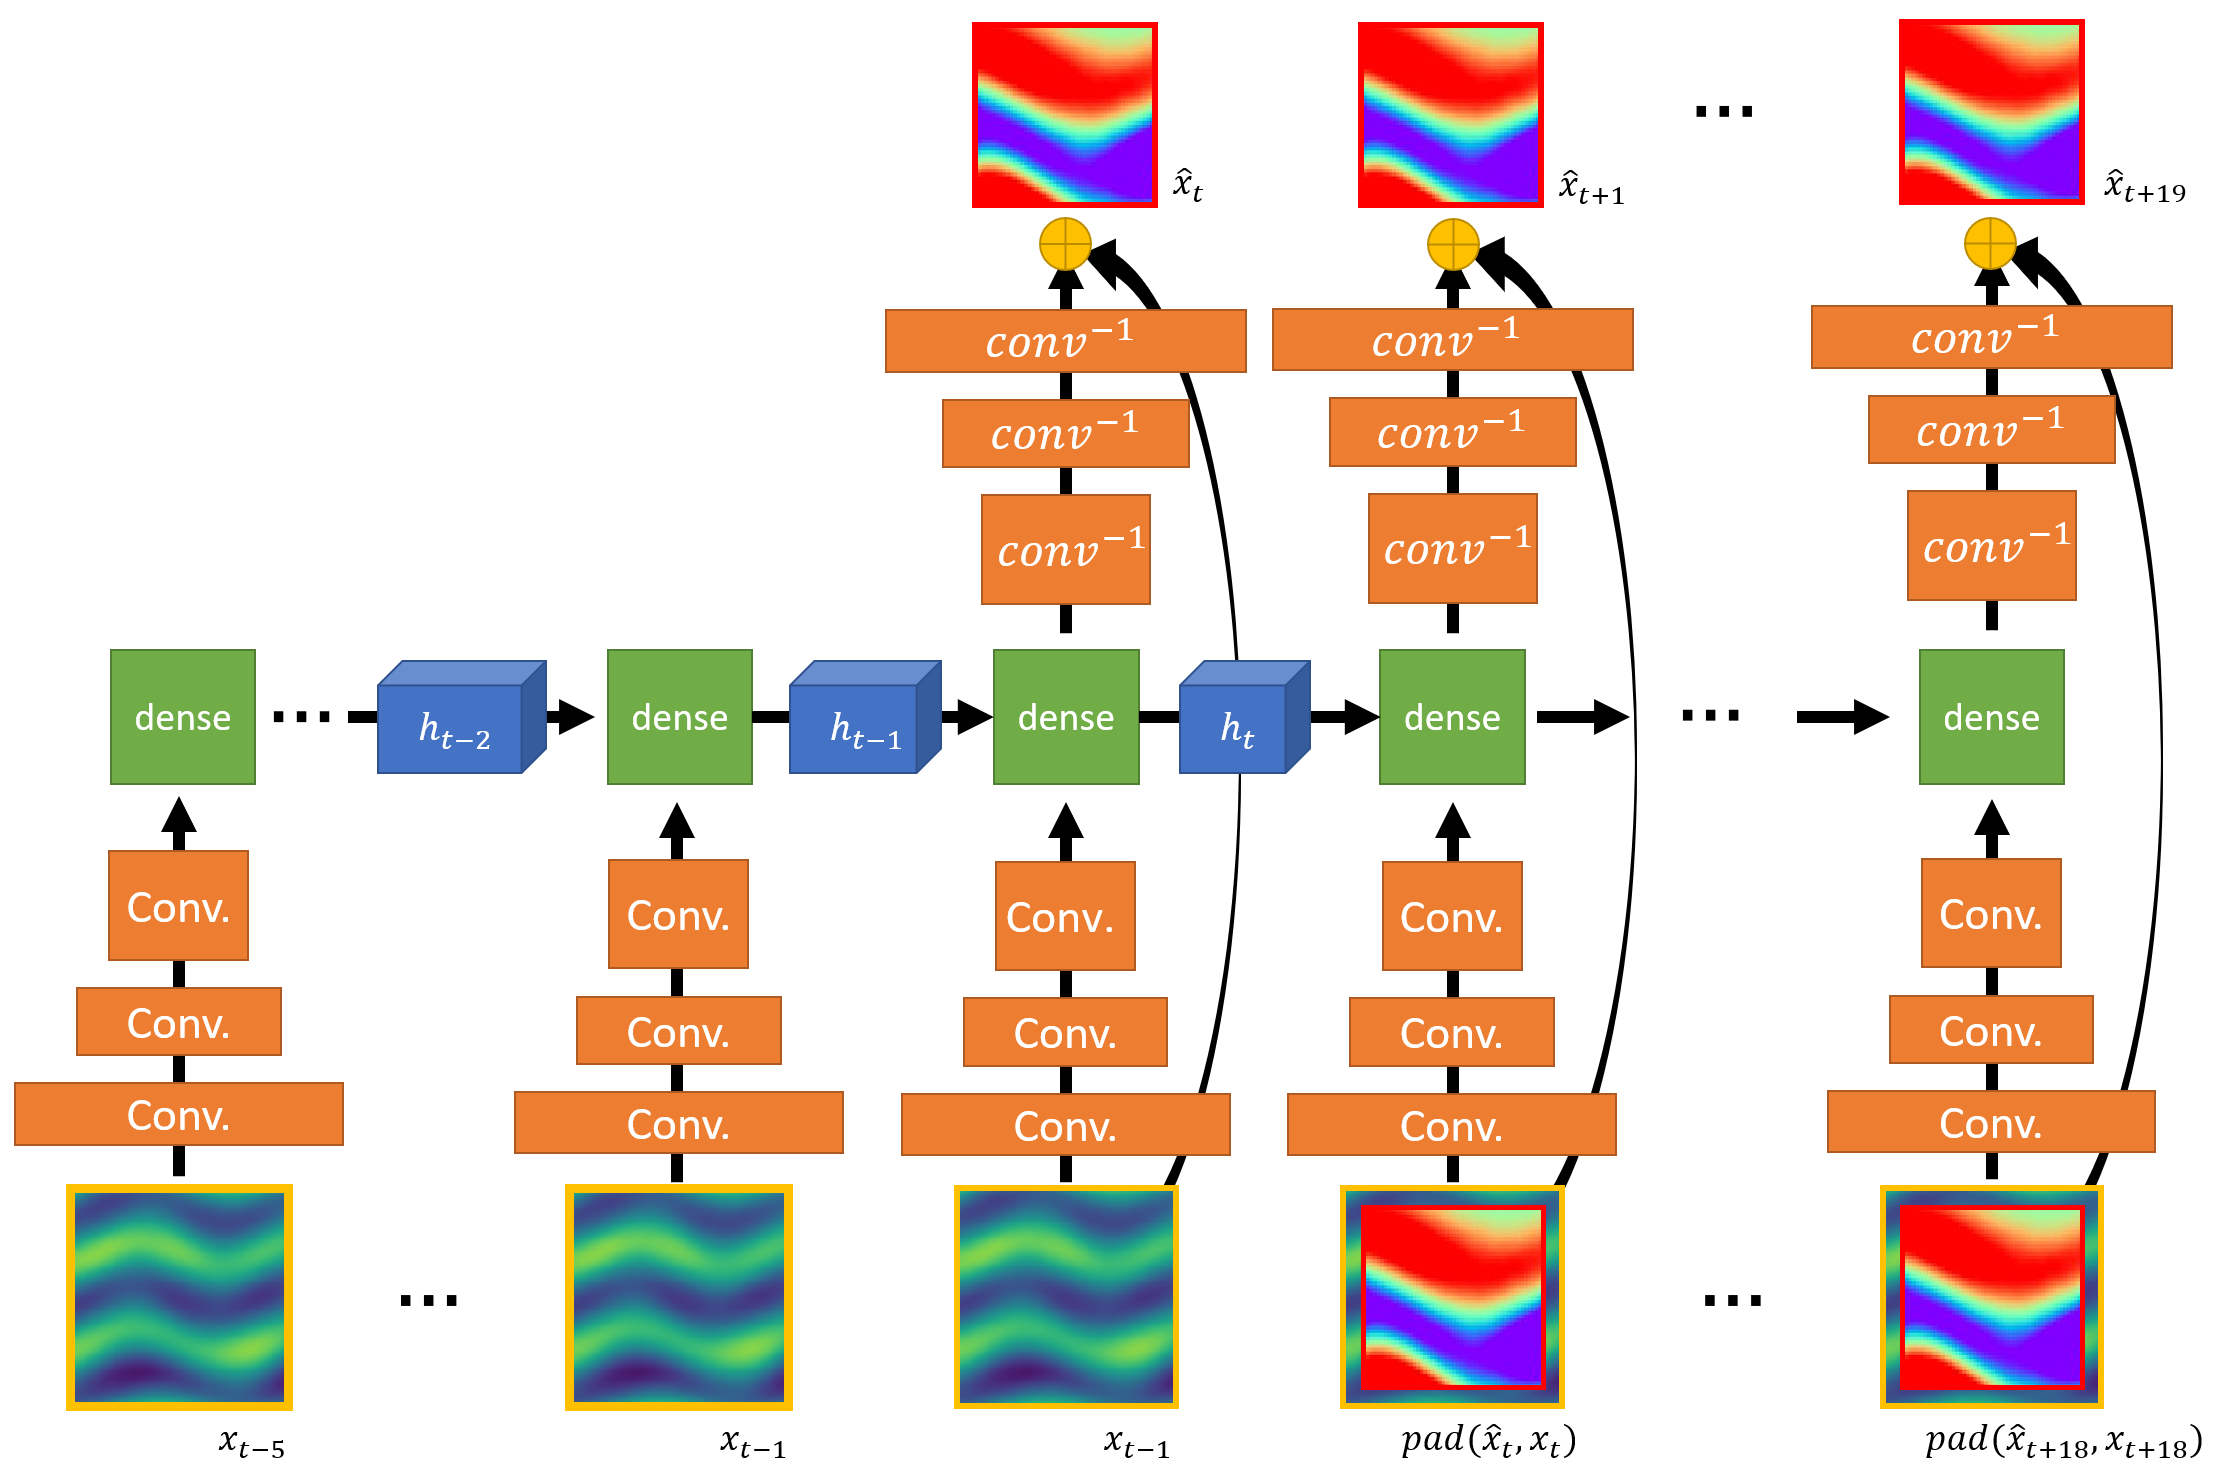
\includegraphics[width=0.7\linewidth]{boundary_aware_arch}
	\caption{Illustration of the boundary-aware architecture modification. By including boundary conditions as padding of previous predicted flow, the dynamics are grounded by the surrounding vorticity resulting in significant reduction in error across the prediction trajectory. This architecture differs slightly from that of the forward-Euler based architectures in that instead of learning the dynamics of the feature space state representation $f(u_t)$, this mechanism of boundary constraining requires we learn the dynamics $f(x_t) = x_{t+1}$ directly.}
	\label{fig:boundry_aware_arch}
	
\end{figure}


Consider learning a PDE of the form $u_t = f(u)$. The simplest approximation of $u_t = f(u)$ is to discretize the time derivative $u_t$ by $\frac{u_{n+1} - u_n}{\bigtriangleup t}$ and approximate the right hand side by $f(u_n)$. This leads to the discrete forward Euler scheme:

$$u_{n+1} = u_n + \bigtriangleup t f(u_n) \label{eqn:ode} $$

where $f(u_n)$ is approximated by a deep neural network. In the previous forward-Euler formulations \textcolor{blue}{, illustrated in figures \ref{fig:arch} and \ref{fig:arch_multi}}, instead of learning the dynamics of the system directly, we use a learned feature representation $u_n$ composed of linear convolutions of the input history. In contrast, for boundary-aware architectures, in order to effectively incorporate the boundary state, we learn directly the vorticity dynamics $f(x_t) = x_{t+1}$ 

In the newly introduced boundary-aware architecture shown in figure \ref{fig:boundry_aware_arch} we utilize a padded activation to learn region dynamics, predicting a 50x50 patch padded to 64x64 to incorporate local state. The down-sampling network uses a series of four convolutions, each with a stride of 2 and a filter-size of 4 doubling the number of channels at each stage. This results in a 8x8x128 vector which we concatenate with the previous hidden state $h_{t}$ and use a dense, fully-connected layer outputting $h_{t+1}$ and the activation used as input to the de-convolution stage. We then up-scale the modified activation using mirrored de-convolutions corresponding with the original down-sampling convolutions. Finally, we utilize a skip-layer as in our forward-Euler architecture, adding the learned dynamics $f(x_t)$ to the previous state, $x_t$ giving us $x_{t+1}$ This model is trained over 20 consecutive time-steps using 5 frames of history to generate the initial hidden state of 64 features using the MSE loss, $L_{mse} = \frac{1}{N}\sum_{t=1}^{n}(y_t - \hat{y_t})^2$. Training is conducted over 40000 batches using the Adam optimizer.


\begin{figure}
	\centering
	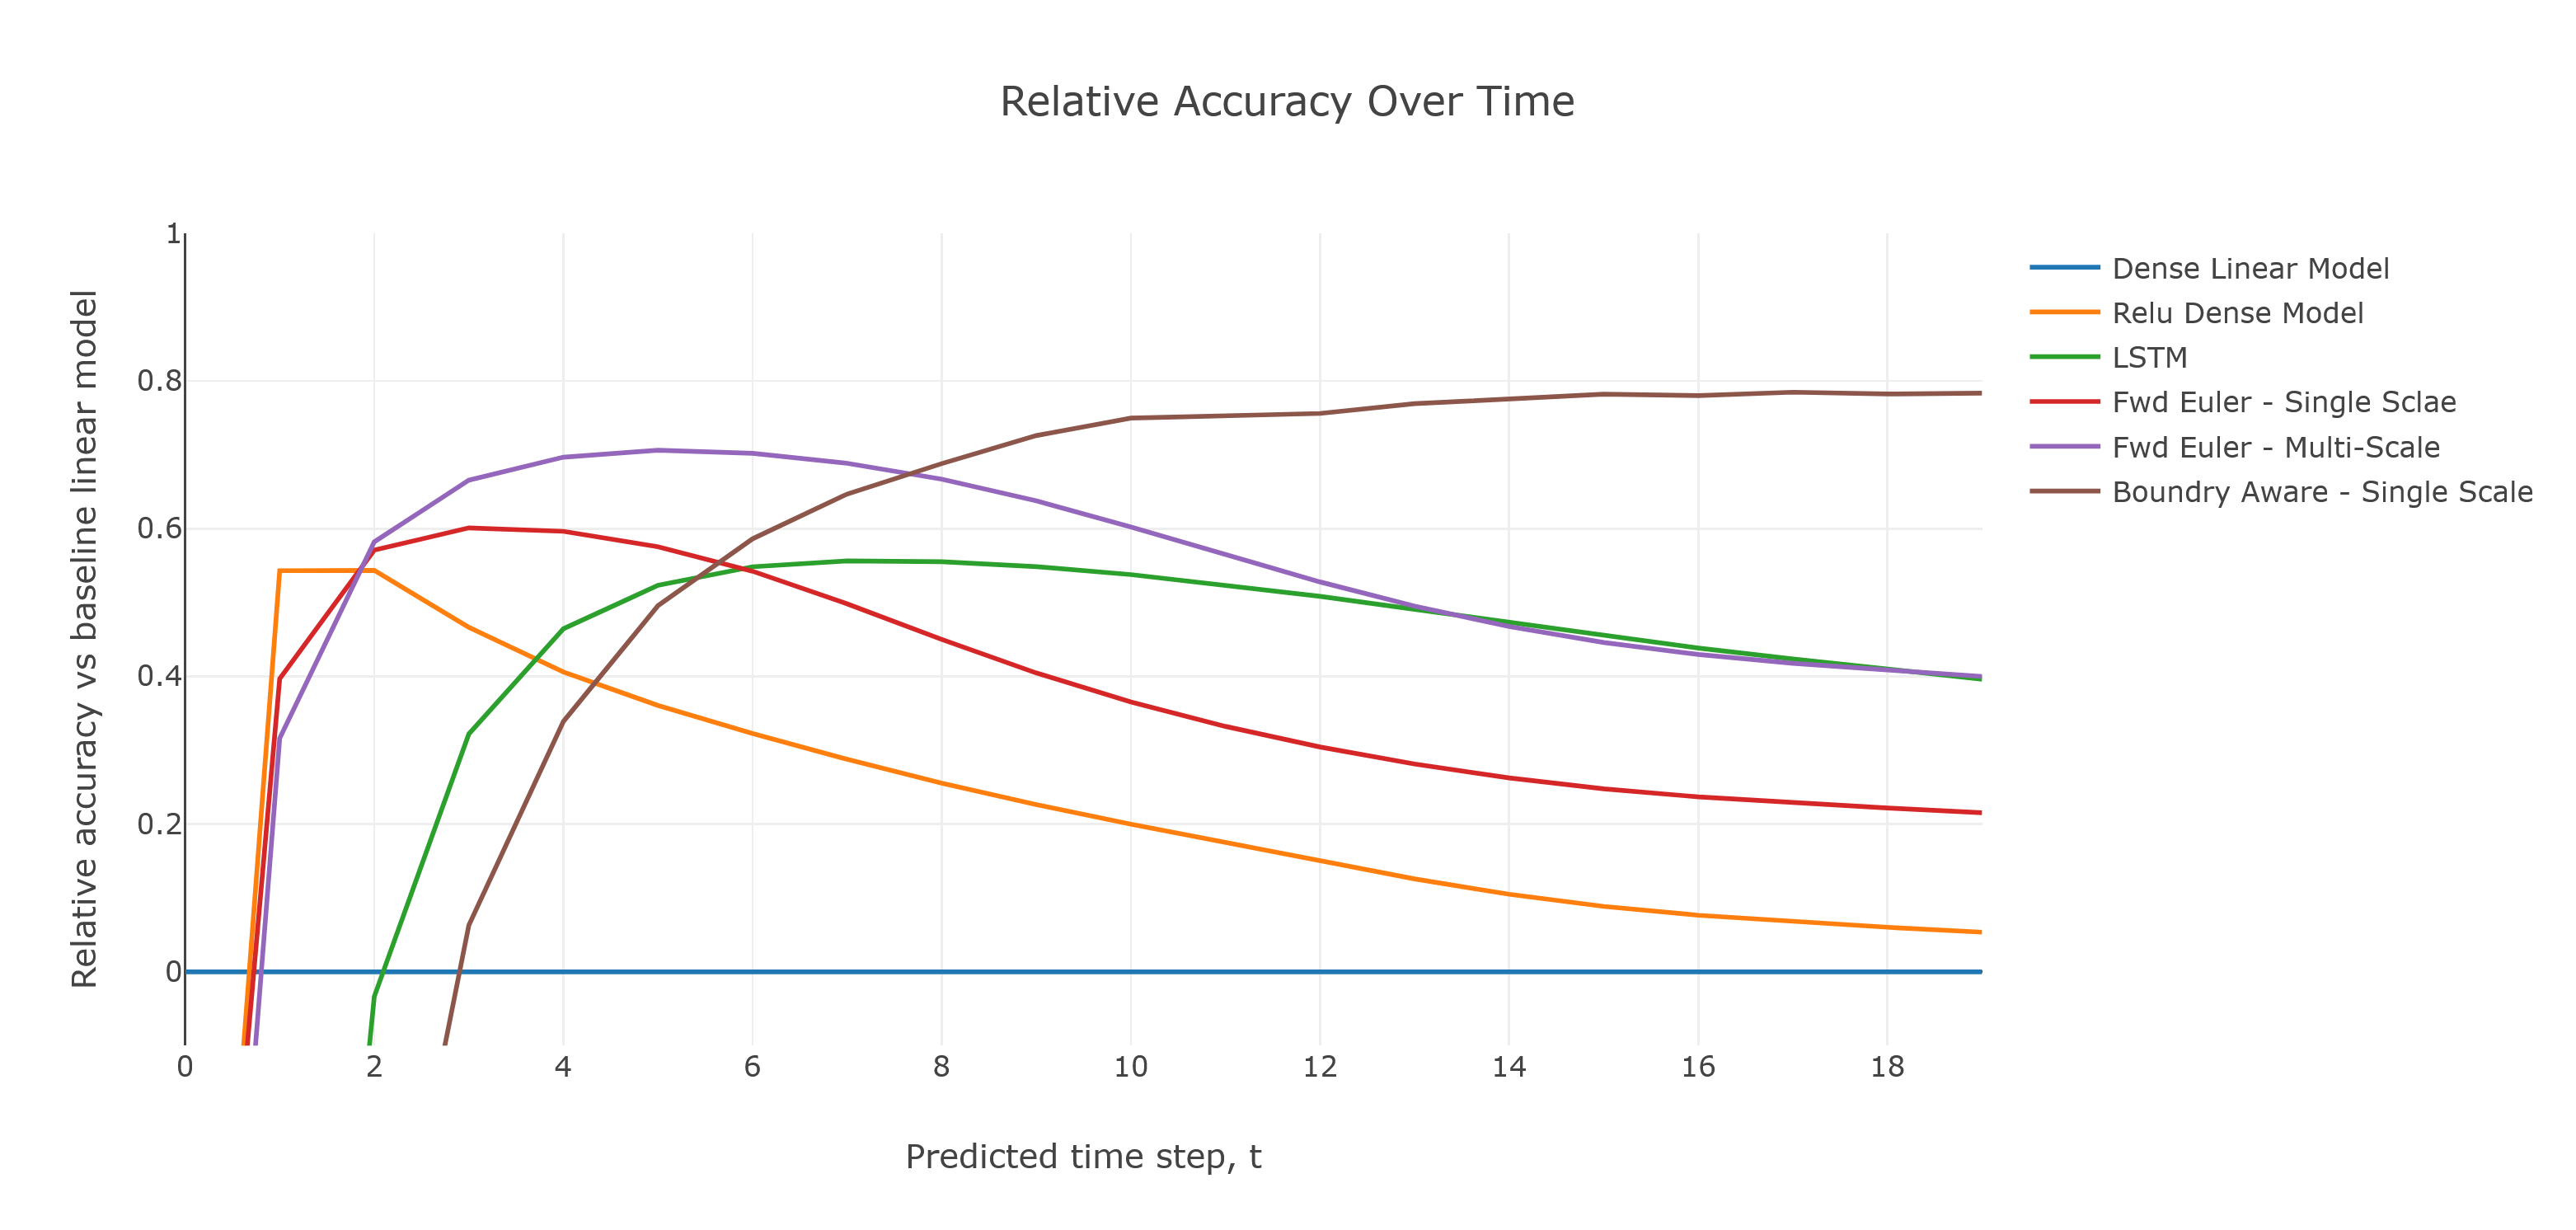
\includegraphics[width=0.95\linewidth]{relative_perf_boundry_aware}
%	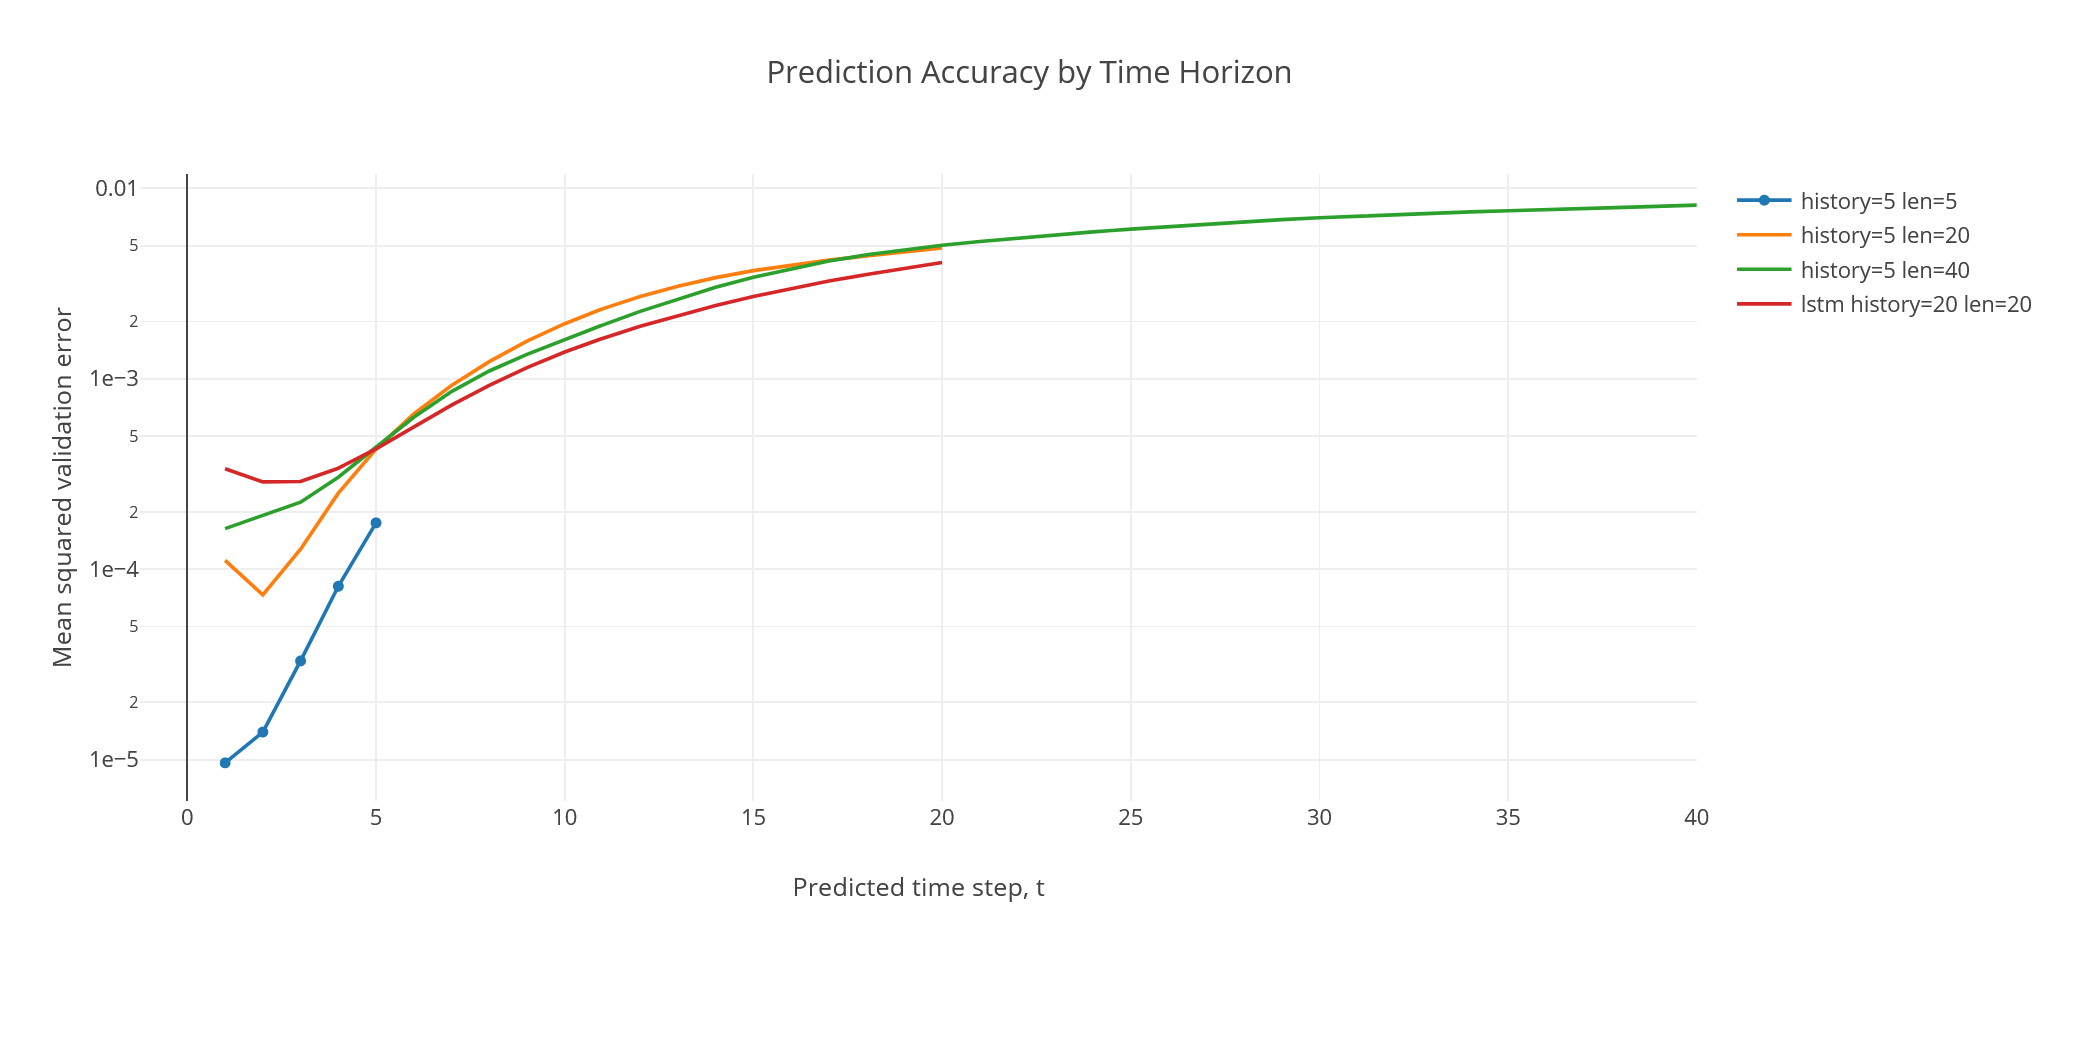
\includegraphics[width=0.9\linewidth]{pde_perf_linear}
	\caption{\small Accuracy of models relative to linear baseline (6.25 million parameters). Relative baseline accuracy, $RBA$, of 1.0 represents perfect prediction for a given time-step, negative values indicate worse than baseline accuracy.}
	\label{fig:abs_perf_new}
\end{figure}



\end{document}

